\documentclass{article}
\usepackage{graphicx}
\usepackage{amsmath}
\usepackage{amsfonts}
\usepackage[parfill]{parskip}
\usepackage{hyperref}
\usepackage[useregional]{datetime2}
\usepackage[toc,page]{appendix}

\usepackage{biblatex}
\addbibresource{references.bib}

\usepackage[T1]{fontenc}
\usepackage{tgbonum}

\usepackage{listings}
\usepackage{xcolor}

\usepackage{longtable}
\usepackage{float}

\usepackage{multirow}

% Define a custom color
\definecolor{backcolour}{rgb}{0.95,0.95,0.92}
\definecolor{codegreen}{rgb}{0,0.6,0}

% Define a custom style
\lstdefinestyle{myStyle}{
    backgroundcolor=\color{backcolour},   
    commentstyle=\color{codegreen},
    basicstyle=\ttfamily\footnotesize,
    breakatwhitespace=false,         
    breaklines=true,                 
    keepspaces=true,                 
    numbers=left,       
    numbersep=5pt,                  
    showspaces=false,                
    showstringspaces=false,
    showtabs=false,                  
    tabsize=2,
}

% Use \lstset to make myStyle the global default
\lstset{style=myStyle}

\graphicspath{ {./figures/} }

\title{ELEC-E5510: Speech Recognition\\
    \large Project report: Multimodal Emotion Recognition in Conversations}
\author{Cuong Nguyen (101559968)}

\newcommand{\inlinemaketitle}{{\let\newpage\relax\maketitle}}

\def\sectionautorefname{Section}

\begin{document}

\inlinemaketitle
\tableofcontents
% \newpage

% \listoffigures
% \newpage

% Content of report would be written here
% \include{./tex/task1.tex}
% ...
% \include{./tex/task2.tex}
\include{tex/intro.tex}
\include{tex/methods.tex}
\include{tex/experiments.tex}
\section{Results}
The experiments evaluated the performance of emotion recognition models using three different modality combinations: unimodal, bimodal, and trimodal approaches. The key metrics for evaluation were weighted F1-score and accuracy. The following summarizes the results for each modality combination:

\subsection{Summary Table}
\begin{table}[h!]
\centering
\begin{tabular}{|c|l|c|c|}
\hline
\textbf{Type} & \textbf{Modality Combination} & \textbf{Weighted F1-score} & \textbf{Accuracy (\%)} \\ \hline
\multirow{3}{*}{Unimodal} & Audio                         & 43.55             & 48.85                 \\ \cline{2-4}
                          & Visual                        & 35.35             & 44.75                 \\ \cline{2-4}
                          & Text                          & 57.52             & 59.77                 \\ \hline
\multirow{3}{*}{Bimodal}  & Audio-Visual                  & 45.25             & 48.24                 \\ \cline{2-4}
                          & Text-Audio                    & 57.61             & 59.39                 \\ \cline{2-4}
                          & Text-Visual                   & 57.51             & 60.15                 \\ \hline
Trimodal                  & Text-Audio-Visual             & 57.88             & 60.61                 \\ \hline
\end{tabular}
\caption{Performance summary across different modality combinations.}
\label{tab:results}
\end{table}

The results summarized in Table~\ref{tab:results} demonstrate that integrating multiple modalities improves emotion recognition performance. While unimodal models showed reasonable accuracy, they struggled to capture the full complexity of emotional cues. Bimodal combinations, particularly those involving text, provided marginal improvements over their unimodal counterparts. The trimodal fusion \emph{(Text-Audio-Visual)} achieved the highest accuracy and F1-score, reflecting the benefits of leveraging complementary information across all three modalities.

\subsection{Confusion Matrices and Class Performance}
The confusion matrices reveal that dominant classes like \textit{Neutral} (Class 0) and \textit{Happy} (Class 1) consistently achieved high recall across all modalities due to their abundance in the dataset. In contrast, underrepresented emotions such as \textit{Fear} (Class 2) and \textit{Disgust} (Class 5) exhibited near-zero recall and were frequently misclassified as \textit{Neutral} or \textit{Sadness}. Misclassifications also occurred between similar emotions, such as \textit{Anger} (Class 3) and \textit{Sadness} (Class 4), particularly in unimodal and bimodal setups. While trimodal fusion reduced these ambiguities by leveraging complementary information, categories like \textit{Surprise} (Class 6) still faced confusion, often being misclassified as \textit{Neutral}.

The model's tendency to default to the \textit{Neutral} class when uncertain highlights the impact of dataset imbalance on predictions. Addressing this issue through techniques like class weighting, oversampling, or advanced fusion methods, such as attention mechanisms, could enhance performance on rare and overlapping emotion categories.

The seven confusion figures are presented in the appendices~\ref{fig:confusion_matrices}, illustrating the classification performance across different modalities in the specified order.


\section{Conclusion}
This study explored the effectiveness of multimodal emotion recognition by combining text, audio, and visual data. The results highlight the value of multimodal approaches, with the trimodal configuration (text-audio-visual) achieving the highest performance. However, the improvements over text-only and bimodal models were marginal, suggesting limitations in the early fusion strategy used. Advanced fusion techniques like attention mechanisms may better exploit inter-modal interactions.

The text modality proved to be the most reliable, both alone and in combination with other modalities, reflecting its richness in conveying emotional cues. In contrast, underrepresented emotions like \textit{Fear} and \textit{Disgust} showed near-zero recall and precision due to dataset imbalance. These findings emphasize the need for class balancing techniques, such as weighted loss functions or data augmentation, to improve the recognition of rare emotions.

Misclassifications between similar emotions, such as \textit{Anger} and \textit{Sadness}, further underscore the limitations of the current feature extraction methods. The model's bias toward the dominant \textit{Neutral} class, influenced by dataset imbalance, also points to the need for more balanced datasets and context-aware modeling.

In summary, while multimodal systems show promise, challenges remain in inter-modal fusion, class imbalance, and generalizability. Future work should focus on improving fusion strategies, addressing dataset limitations, and leveraging advanced architectures to enhance the robustness and applicability of emotion recognition models.

\section{Division of labor}
\begin{itemize}
    \item Cuong Nguyen:
        \begin{itemize}
            \item Wrote experiment code.
            \item Wrote `Literature Study' and `Experiments' sections.
        \end{itemize}
    \item Raihan Gafur:
        \begin{itemize}
            \item Wrote classification matrices code.
            \item Wrote `Results' and `Conclusion' sections.
        \end{itemize}
\end{itemize}
\include{tex/ack.tex}


\printbibliography[heading=bibintoc]

% \newpage
\begin{appendices}
	\section{Code}
All code is publicly accessible at \url{https://github.com/ancuongnguyen07/Multimodal-ERC/tree/master/code}

\begin{lstlisting}[label={lst:training-script},caption=Running the training script.]
python train_MELD.py --features-type text_audio_visual \
    --data-path data/MELD_features_raw1.pkl --output-dir models/
\end{lstlisting}

\begin{lstlisting}[label={lst:testing-script},caption=Running the testing script.]
python test_MELD.py --model-path ../models/text_audio_visual_BiDi_Att.pth \
    --features-type text_audio_visual
\end{lstlisting}

\section{Confusion Matrices}
\begin{figure}[htbp]
    \centering
    \begin{subfigure}[b]{0.45\textwidth}
        \centering
        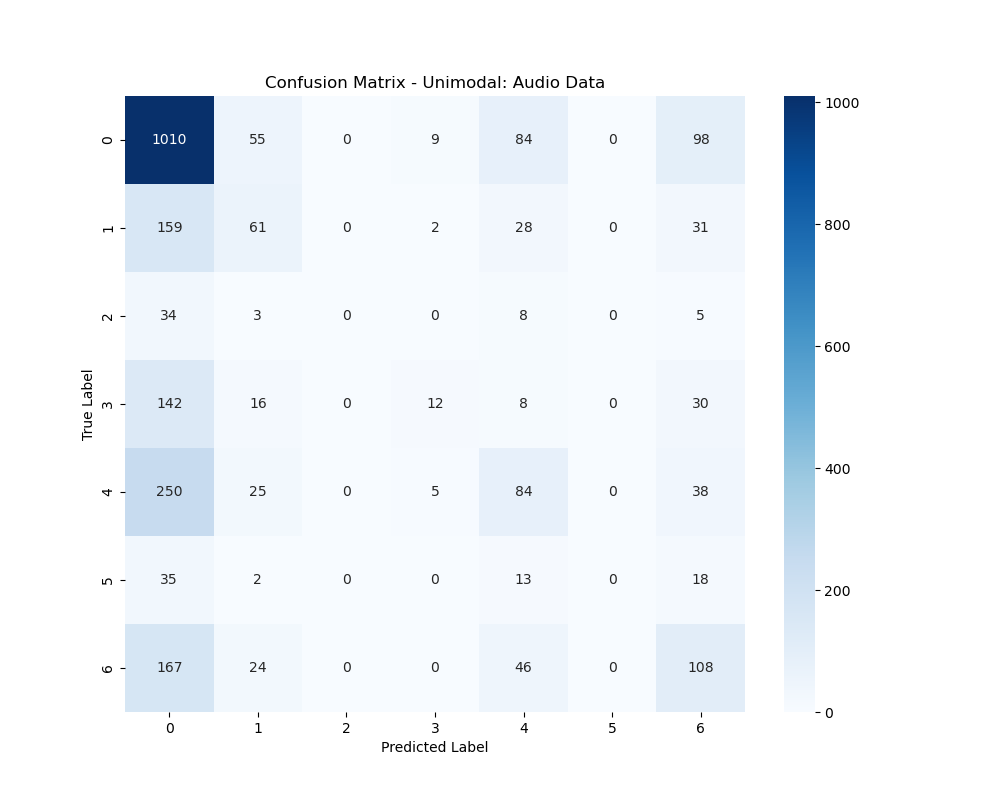
\includegraphics[width=\textwidth]{figures/audio.png}
        \caption{Unimodal: Audio Data}
    \end{subfigure}
    \hfill
    \begin{subfigure}[b]{0.45\textwidth}
        \centering
        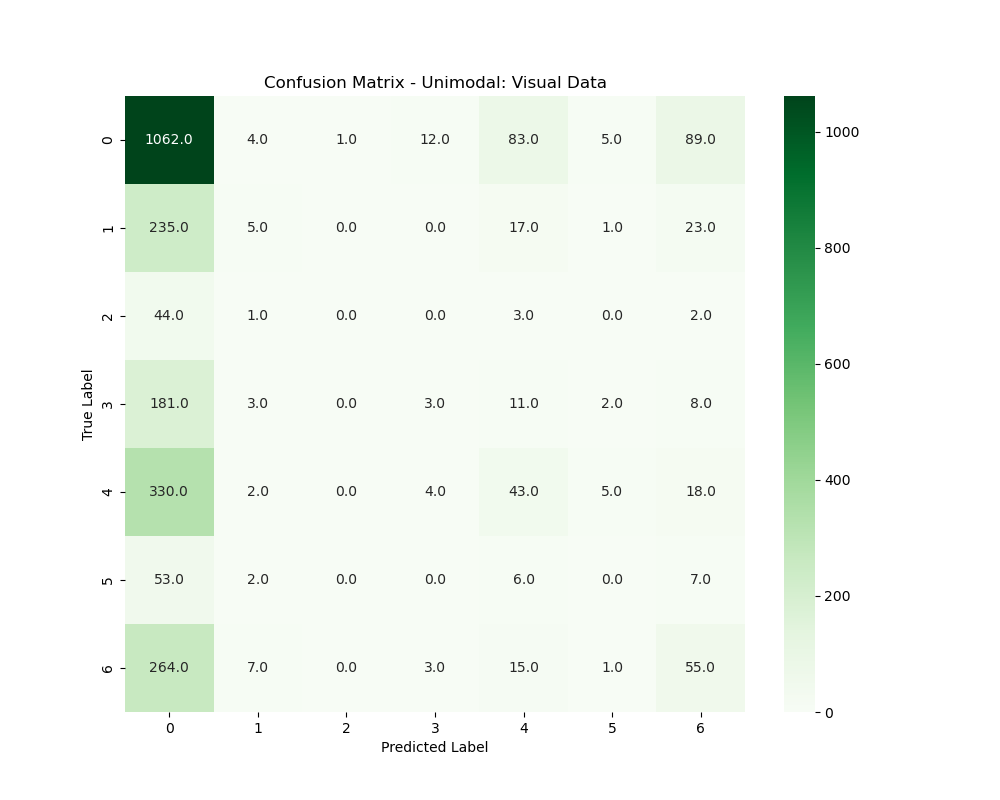
\includegraphics[width=\textwidth]{figures/visual.png}
        \caption{Unimodal: Visual Data}
    \end{subfigure}

    \vspace{0.5cm} % Vertical space between rows

    \begin{subfigure}[b]{0.45\textwidth}
        \centering
        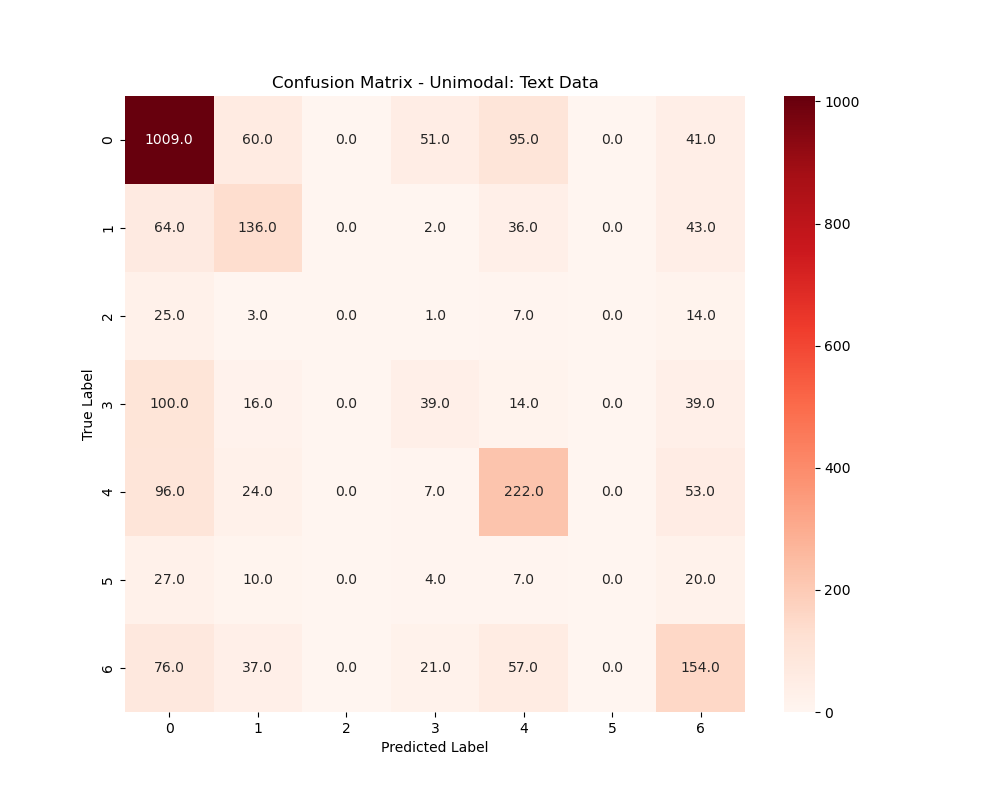
\includegraphics[width=\textwidth]{figures/text.png}
        \caption{Unimodal: Text Data}
    \end{subfigure}
    \hfill
    \begin{subfigure}[b]{0.45\textwidth}
        \centering
        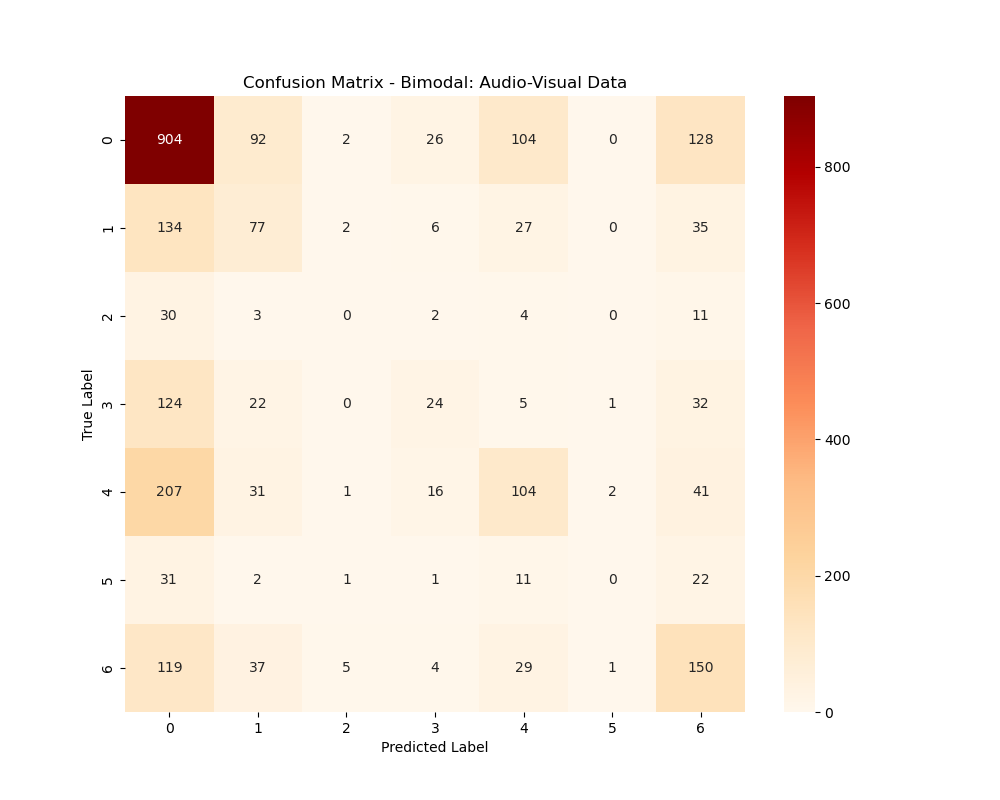
\includegraphics[width=\textwidth]{figures/audio-visual.png}
        \caption{Bimodal: Audio-Visual Data}
    \end{subfigure}

    \vspace{0.5cm} % Vertical space between rows

    \begin{subfigure}[b]{0.45\textwidth}
        \centering
        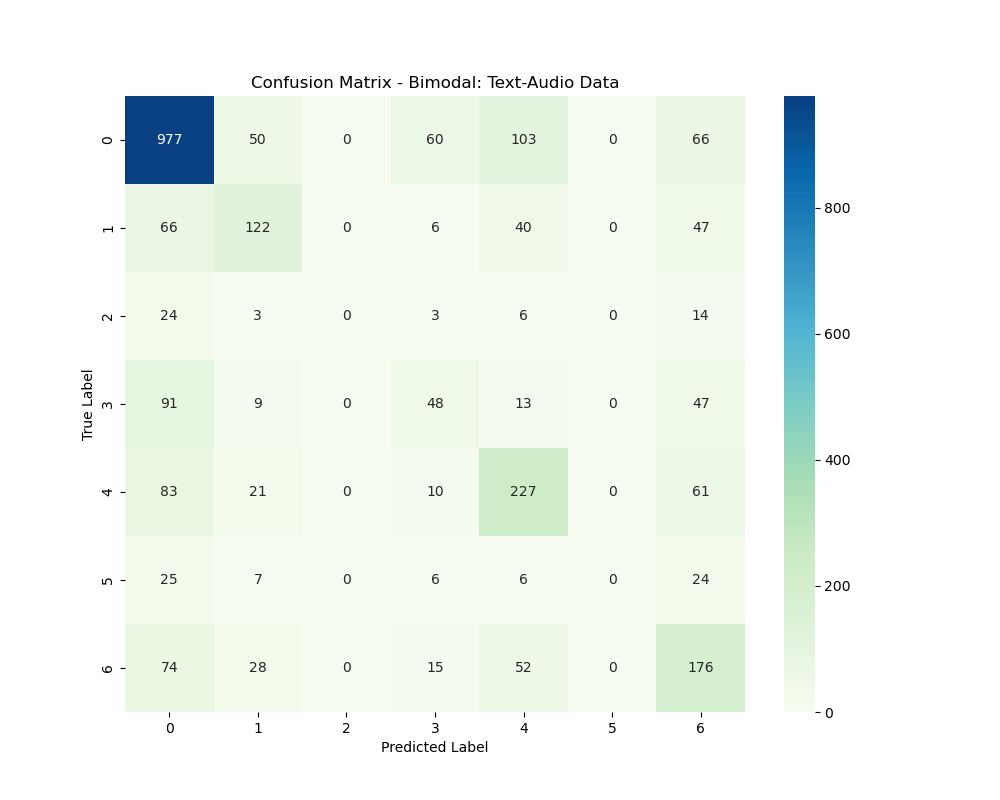
\includegraphics[width=\textwidth]{figures/text-audio.png}
        \caption{Bimodal: Text-Audio Data}
    \end{subfigure}
    \hfill
    \begin{subfigure}[b]{0.45\textwidth}
        \centering
        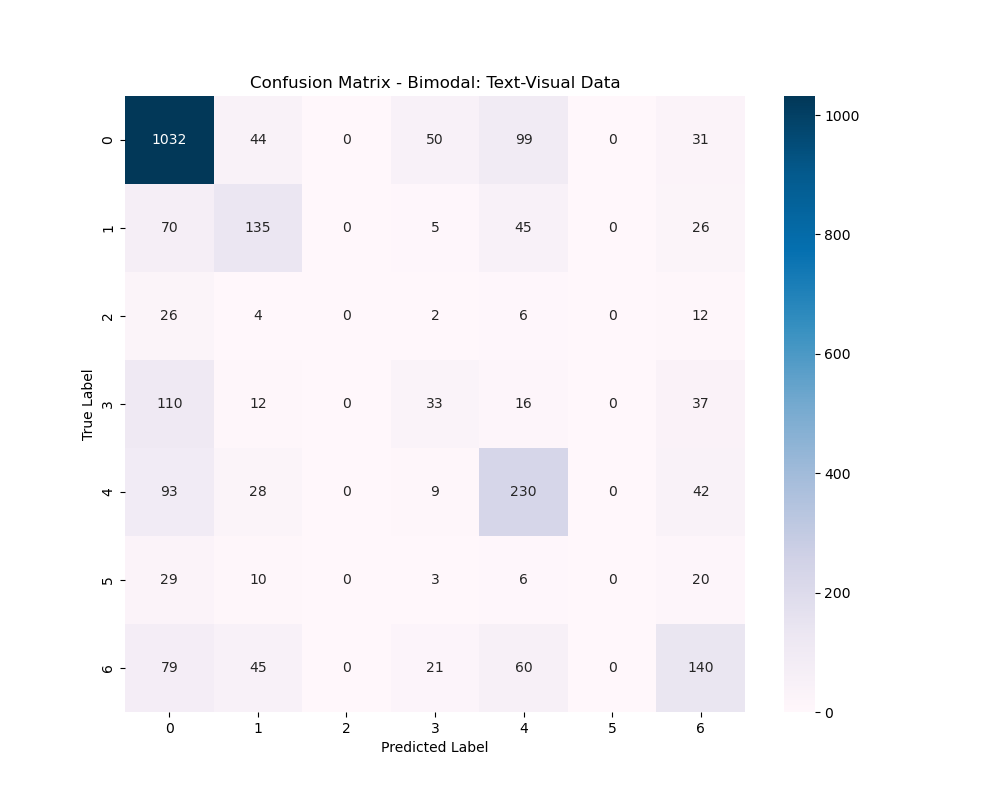
\includegraphics[width=\textwidth]{figures/text-visual.png}
        \caption{Bimodal: Text-Visual Data}
    \end{subfigure}

    \vspace{0.5cm} % Vertical space between rows

    \begin{subfigure}[b]{0.45\textwidth}
        \centering
        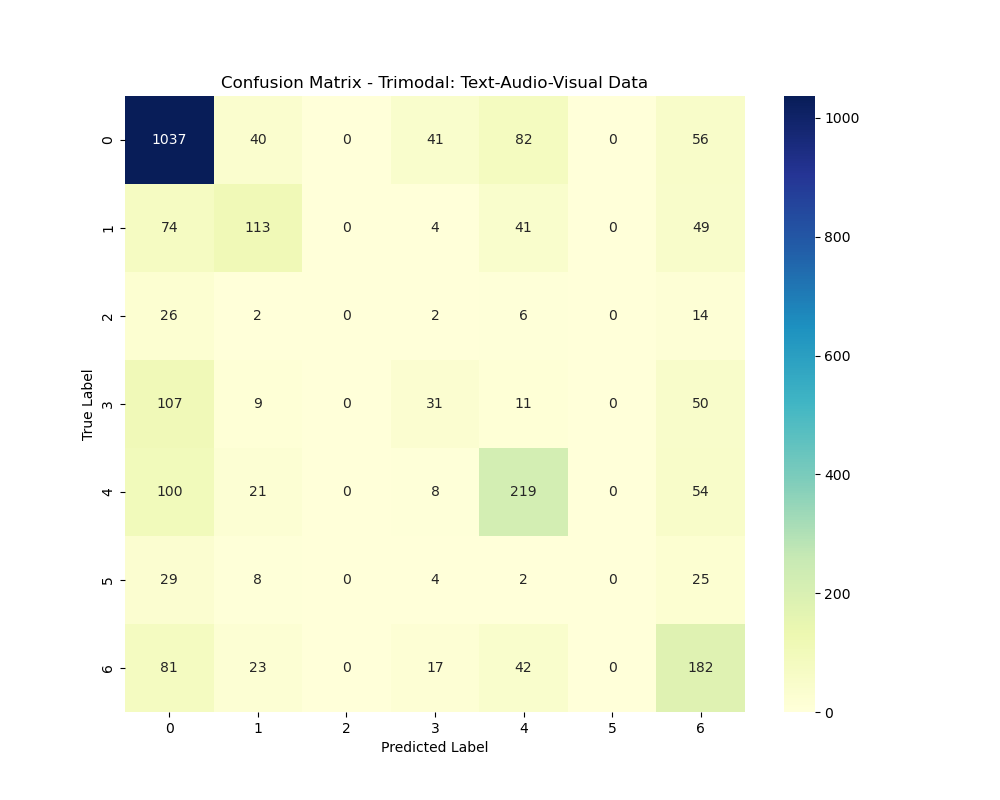
\includegraphics[width=\textwidth]{figures/text-audio-visual.png}
        \caption{Trimodal: Text-Audio-Visual Data}
    \end{subfigure}

    \caption{Confusion Matrices Across Modalities}
    \label{fig:confusion_matrices}
\end{figure}
\end{appendices}

\end{document}
